\section{Data Visualization}
\label{data-visualization}

The objective of data visualization is to live debug and tune both hardware gain
and algorithms control constants. The ideal case is to have both real time chart
as well as a buffered/triggered one, essentially something like an oscilloscope.
That has to be performant for real time audio signals, sampled at more than 47 kHz.

There are a great amount of JavaScript DOM libraries for charting, but most of
them are too automatic or have too much details, making them too slow for the project need.
The solution was to build an own library for that, again available as an open source
project at both GitHub and npm \cite{react-plotter}.

\subsection{Requirements}
\label{data-visualization-requirements}
\begin{itemlist}
  \item Be a React Component
  \item Automatic calculations for array input
  \item Option for triggering
  \item Option for buffering
  \item Minimum Redraw
  \item Fixed Height/Width
\end{itemlist}

\subsection{Algorithm}
Triggering and buffering are achieved by using a filter that only calls the plotting
function when the options are met. This filter is simply the function called to
add data, and it is represented by \autoref{react-plotter-add-diagram}. 

\begin{figure}[htb]
  \caption{Add Function Diagram}
  \label{react-plotter-add-diagram}
  \centering
  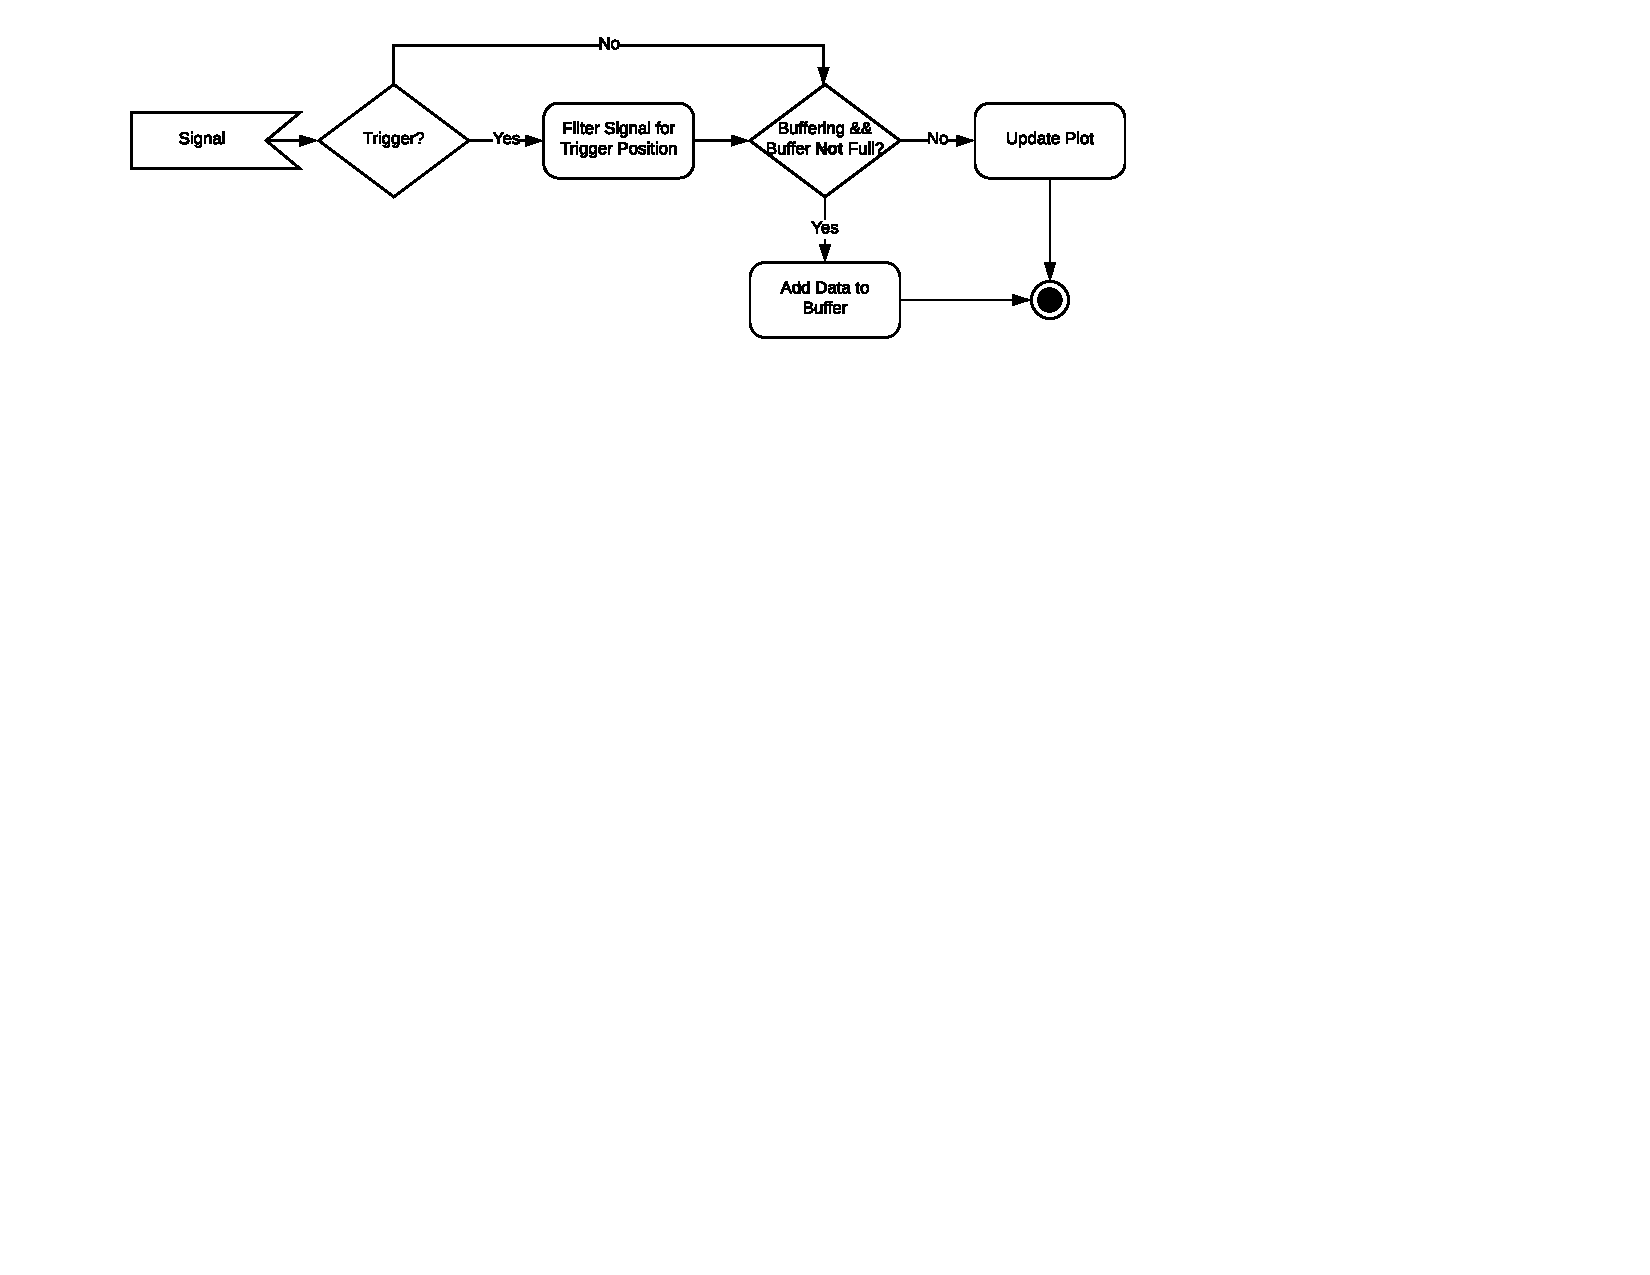
\includegraphics[scale=0.9]{images/react-plotter-add-diagram}
  \legend{Source: authors}
\end{figure}
For the actual drawing a triple buffer technique is used, one for holding the last
state (called plotBuffer), on for drawing (called drawingBuffer) and finally the
one actually rendered (called canvas). That last one is needed so the arrows don't
get saved on the drawing scene. 

For linear plot time a translation is established, in a way that only the new
points will be drawn, the past ones are only translated to the left. The steps
of the algorithm are as follow:
\begin{enumerate}
  \item Clear drawingBuffer
  \item Copy plotBuffer to drawingBuffer translating (removing) extra data
  \item Draw new data on drawingBuffer
  \item Copy drawingBuffer to plotBuffer
  \item Copy plotBuffer to canvas
  \item Draw arrows on canvas
\end{enumerate}

\subsection{Implementation}
Using the listed requirements (\autoref{data-visualization-requirements}) a minimum
API was built as a React component. Being such all it gives is a set of properties,
for which the chart is drawn (when needed), they are listed in \autoref{react-plotter-props}.
\begin{table}[htb]
  \ABNTEXreducedfont
  \caption[React Plotter Props]{React Plotter Props}
  \label{react-plotter-props}
  \centering
  \begin{tabular}{c|c|c}
    \textbf{Property} & \textbf{Type} & \textbf{Description} \\
    \hline \hline
    style &	Function & Style function (called to print the data) \\
    \hline
    {[trigger]} &	number & Use trigger \\
    \hline
    {[onlyFull=true]}	& bool & When using trigger it tells if the view should \\
                      &      & wait for a complete data set before updating \\
    \hline
    {[width=300]} &	number \\
    \hline
    {[height=150]} & number \\
    \hline
    {[initialData=[ ]]} & number{[ ]} \\
    \hline
    {[appendData=[ ]]} & number{[ ]} \\
    \hline
    {[dataSize=100]} & number \\
    \hline
    {[pixelSkip=1]} &	number &	Pixels between points \\
    \hline
    {[max=100]} &	number & Maximum Y Value \\
    \hline
    {[min=-100]} & number & Minimum Y Value \\
    \hline
    {[useMean=true]} & bool & Use mean calculation, otherwise median  \\
  \end{tabular}
  \legend{Source: \citeonline{react-plotter}}
\end{table}
The style property is a function that is called to render each point. Two styles
were built, a line plot (points are connected by a straight line) and a digital
plot (digital signal standard chart, not used in the final version of this project).

\subsection{Results}
The results are more than satisfactory, tested to be able to run multiple plots
of audio speed signals at the same time without much effort. \autoref{plot-real-time}
and \autoref{plot-triggered} show how the visualization looks on the
project, but full details and working examples are also available at GitHub
\cite{react-plotter}.

\begin{figure}[htb]
 \centering
  \begin{minipage}{0.4\textwidth}
    \centering
    \caption{Real Time Plot} \label{plot-real-time}
    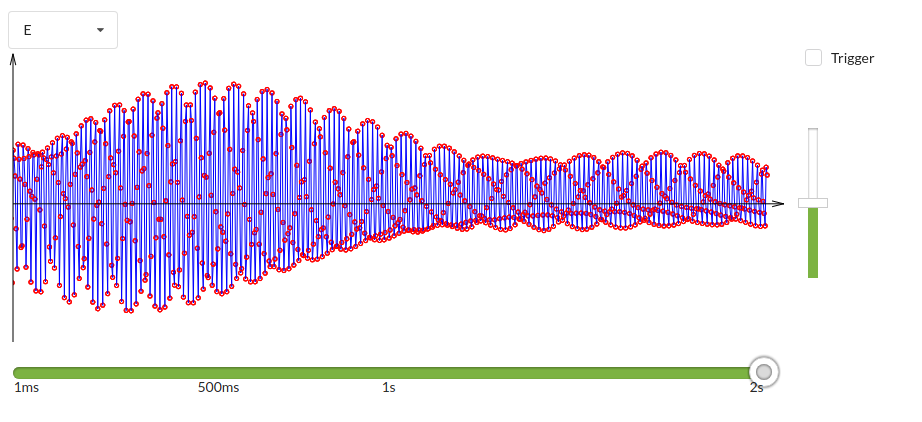
\includegraphics[scale=0.22]{images/snapshots/plot-real-time}
    \legend{Source: authors}
  \end{minipage}
  \hfill
  \begin{minipage}{0.4\textwidth}
    \centering
    \caption{Triggered Plot} \label{plot-triggered}
    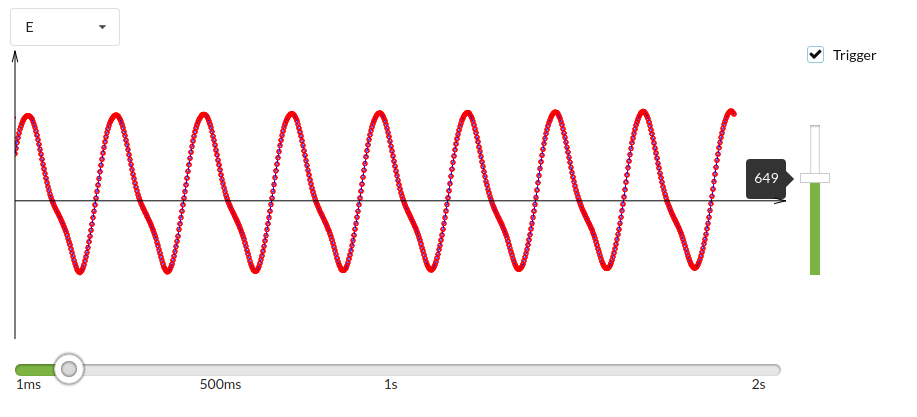
\includegraphics[scale=0.22]{images/snapshots/plot-trigger-E}
    \legend{Source: authors}
  \end{minipage}
\end{figure}
